\chapter{Conception du pipeline de données}
\section{Définir les objectifs de l'application}

L'outil produit dans le cadre de mon stage de Master 2 au Département de l'administration des données des Archives nationales est une application ayant pour fonction la fabrication de paquets d’archives (SIP) pour la reprise des reportages photographiques de la Présidence de François Hollande en vue de leur versement dans le SAE Vitam des Archives nationales. Baptisée ORPhÉE (Outil de Reprise de Photographies et Éléments Embarqués), son intérêt principal réside en sa capacité à extraire les métadonnées internes des photographies, notamment les métadonnées descriptives qui ont pu être renseignées par le photographe (description, mots-clés, nom du photographe, lieux de la prise de vue). Le deuxième enjeu était de s'assurer que l'application permettait bien de restituer l'arborescence des reportages après leur versement. 

ORPhÉE devait donc produire un bordereau de versement conforme au SEDA (manifest) restituant la structure intellectuelle des reportages et enrichi des métadonnées internes des photographies et des métadonnées externes des reportages issues de l'export CSV de la base Cindoc des archives de l'Élysée. La création du manifest devait s'accompagner de la copie à plat et du renommage de l'ensemble des fichiers ajoutés au paquet dans un dossier \enquote{content}. 

La majeure partie de mon travail a consisté en la création du manifest : c'est en effet lui qui fournira au SAE les informations de structure et de description qui permettront l'affichage et l'accessibilité des fichiers archivés. Une brève présentation de la structure d'un manifest semble donc de rigueur afin de comprendre au mieux le processus de création de l'application ORPhÉE. Cette structure est synthétisée par la Figure 8.1 à la page suivante.

\begin{figure}
	\centering
	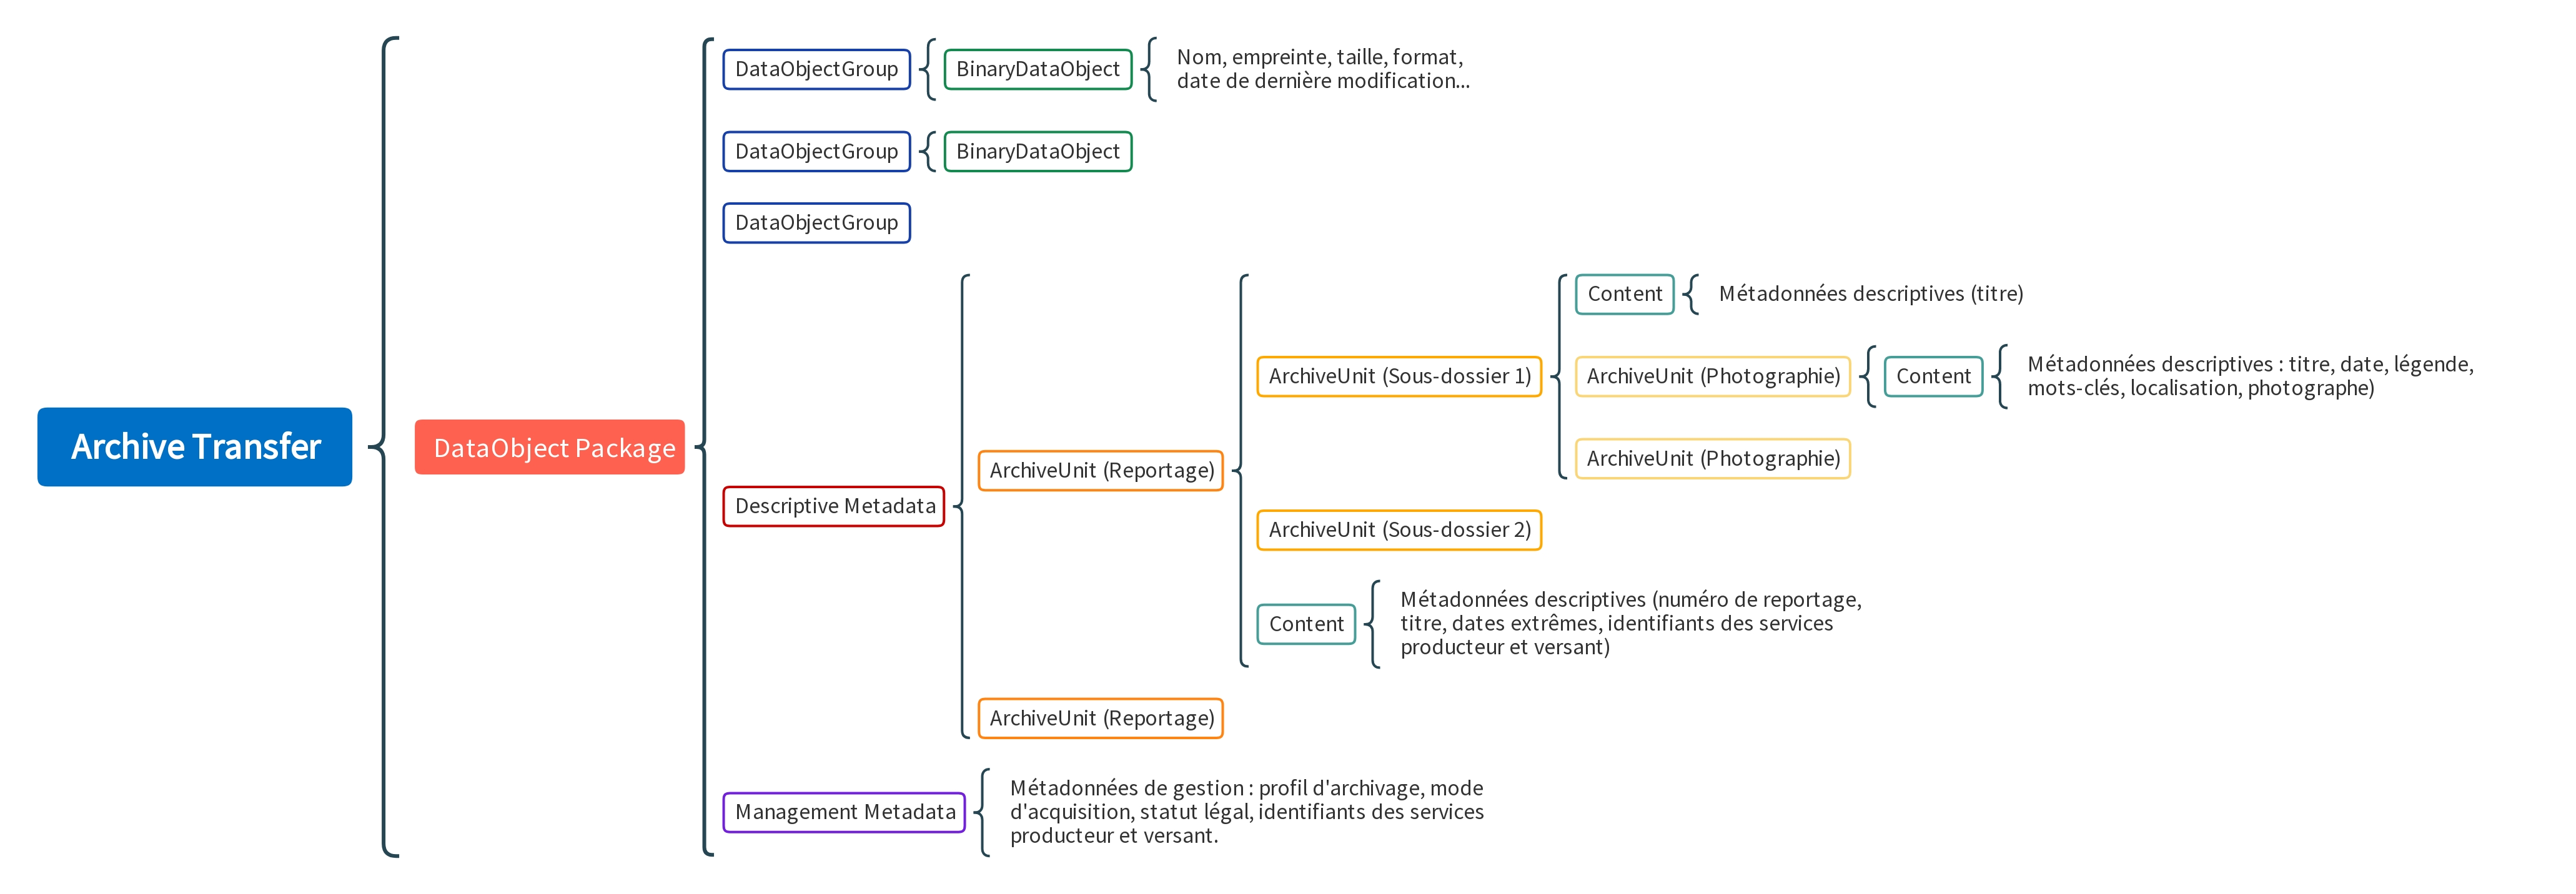
\includegraphics[angle=90, height=\dimexpr\textheight-2cm\relax]{./img/ArchiveTransfer.jpg}
	\caption{Schéma présentant les principales sections du manifest en SEDA produit par l'application ORPhÉE, ainsi que leur contenu.}
\end{figure}

\newpage
Le manifest est un document XML dont la racine est l'élément \xmlinline{<ArchiveTransfer>}. Il est composé d'un en-tête qui fournit l'identifiant du paquet d'archives et des informations techniques liées aux modalités de versement, et d'un élément \xmlinline{<DataObjectPackage>} qui contient les métadonnées techniques, descriptives et de gestion relatives aux archives constitutives du paquet. Nous nous intéresserons donc particulièrement au contenu de cet élément. Il se divise en trois grands blocs : une succession d'éléments \xmlinline{<DataObjectGroup>}, un élément \xmlinline{<DescriptiveMetadata>}, et un élément \xmlinline{<ManagementMetadata>}. Chaque \xmlinline{<DataObjectGroup>} correspond à un document dans toutes ses versions (originaux, diffusion, version textuelle). Ainsi, en SEDA, un même document peut être représenté par plusieurs fichiers, chacun étant associé à un élément \xmlinline{<BinaryDataObject>} : dans notre cas, chaque document correspond à un seul fichier, l'original,  chaque \xmlinline{<DataObjectGroup>} est donc composé d'un seul \xmlinline{<BinaryDataObject>}. Cet élément contient des métadonnées techniques relatives au fichier : empreinte, format, date de dernière modification, taille... L'élément \xmlinline{<DescriptiveMetadata>} permet de restituer la structure du versement ainsi que les métadonnées descriptives associées à chaque unité d'archives, ou \xmlinline{<ArchiveUnit>}. L'élément \xmlinline{<ManagementMetadata>} contient quant à lui les métadonnées de gestion communes à l'ensemble du paquet. Pour bien associer chaque \xmlinline{<DataObjectGroup>} à l' \xmlinline{<ArchiveUnit>} correspondant, un jeu d'identifiants est mis en place au sein du manifest. Les fichiers copiés dans le paquet correspondant aux éléments \xmlinline{<BinaryDataObject>}, ils sont renommés en utilisant les identifiants associés à ces éléments.

\section{Fonctionnement de l'application}

\subsection*{Collecte des données et métadonnées nécessaires}
Pour fonctionner correctement, l'application doit ingérer un certain nombre d'informations qui serviront ensuite à enrichir le manifest, à sélectionner les reportages à ajouter au paquet, ou à définir les modalités de rattachement dans le SAE. Certaines informations, communes à tous les paquets de reportages photographiques de la Présidence, sont inscrites \enquote{en dur} dans l'application : l'utilisateur n'a pas besoin de les renseigner. C'est le cas par exemple des métadonnées de gestion du \xmlinline{<ManagementMetadata>}. D'autres informations sont relatives au paquet et sont demandées à l'utilisateur au lancement de l'application : numéro d'entrée, numéro du paquet, méthode de rattachement... Enfin, la plupart des informations sont issues de fichiers externes ou des photographies elles-mêmes.

\subsubsection*{Import des fichiers de données}

L'application prend deux fichiers en entrée : le CSV contenant les métadonnées descriptives externes des reportages, et la liste au format texte des reportages à ajouter au paquet. ORPhÉE transforme l'export CSV de la base Cindoc en listes de données : chaque ligne du tableau correspondant à une liste des métadonnées descriptives de chaque reportage (numéro, titre, dates extrêmes), toutes ces listes sont réunies dans une grande liste qui correspond au fichier CSV dans son ensemble. Le contenu du fichier texte est également transformé en une liste de numéros de reportages : cette liste est utilisée tout au long du traitement pour vérifier à toutes les étapes que seuls les reportages sélectionnés sont inclus au paquet.

\subsubsection*{Extraction des métadonnées internes et calcul des métadonnées de format}

Trois étapes du pipeline permettent l'exploitation des métadonnées internes des fichiers. La librairie PyExiftool est utilisée pour extraire les métadonnées internes des fichiers selon les mêmes modalités qu'Exiftool. La commande Python est par ailleurs très proche de celle utilisée en ligne de commande avec l'application lorsqu'elle est appelée dans le terminal : précision du format attendu pour la restitution des données extraites (JSON), commande d'itérer dans les sous-dossiers du répertoire analysé, liste des métadonnées à extraire, puis chemin du répertoire à analyser (représenté ici par la variable \enquote{item\_path}). J'ai rencontré de nombreux problèmes d'encodage lors de l'extraction des métadonnées, les caractères spéciaux n'étant pas restitués correctement, il était en effet nécessaire d'expliciter à presque chaque étape du pipeline l'encodage des chaînes de caractères manipulées (ici, l'UTF-8).
 \\
\begin{python}
exif_data_list = et.execute_json('-r', '-b', '-FileName', '-CreateDate', '-By-line', '-Artist', '-City', '-Country',
'-Country-PrimaryLocationName', '-Description', '-Subject', '-Keywords', '-FileModifyDate', '-Filesize#', item_path)
\end{python}

Le logiciel Siegfried est ensuite utilisé pour produire les métadonnées de format et calculer l'empreinte, l'ensemble de ces informations est également fourni au format JSON. Les métadonnées collectées au cours de ces deux étapes n'étaient cependant pas réunies au sein d'une même variable JSON, ce qui ralentissait considérablement l'application qui devait parcourir deux sources d'information pour récupérer les métadonnées associées à un même fichier. Pour simplifier ce processus, j'ai ajouté une étape dont l'objectif était de fusionner les deux sources de métadonnées : l'application parcourt d’abord les métadonnées issues de Siegfried et identifie les chemin de tous les fichiers. Elle cherche ensuite le même chemin dans les métadonnées extraites par Exiftool. Lorsqu’une correspondance est trouvée, la fonction fusionne les métadonnées Exiftool et Siegfried pour que l’ensemble des métadonnées d’un même fichier soient stockées au même endroit.
\\

À l'issue de cette première étape, l'ensemble des métadonnées nécessaires a été identifié, extrait et stocké. L'étape suivante d'écriture du manifest permettra des les associer aux objets de données (fichiers) et aux unités archivistiques correspondantes.

\subsection*{Écriture du manifest}
Pour l'écriture des éléments du manifest en XML, j'ai utilisé la librairie Python ElementTree. Elle permet de créer, organiser et écrire des fichiers XML en proposant des outils pour définir des balises, ajouter des sous-éléments, et sauvegarder la structure XML dans un fichier. Dans un premier temps, l’élément racine du manifest et les éléments de l’en-tête sont créés. La majorité d'entre eux ont des valeurs fixes qui sont renseignées directement dans le code de l'application (noms des services producteur et versant, nom du service d'archives). Est ensuite créé l'élément \xmlinline{<DataObjectPackage>} dont le contenu sera écrit petit à petit au cours des étapes successives du pipeline de données.
\subsection*{Identifier les objets de données}

Pour créer les éléments \xmlinline{<DataObjectGroup>} et \xmlinline{<BinaryDataObject>}, l'application parcourt de manière récursive l’ensemble des fichiers des reportages sélectionnés : ces deux éléments sont créés pour chacun des fichiers identifiés. L'application est programmée pour ignorer les fichiers exclus de la reprise (fichiers système ou masqués) repérés à l'aide de leur nommage. Dans un second temps, l'application recherche les métadonnées techniques de ces objets de données calculées par Siegfried et les associe à chaque \xmlinline{<BinaryDataObject>}. Voici un extrait du manifest représentant ces éléments à ce point du traitement. On notera que certaines informations sont absentes à ce stade d'écriture du manifest.

\begin{xml}
<DataObjectGroup>
	<BinaryDataObject>
		<DataObjectVersion>BinaryMaster_1</DataObjectVersion>
		<Uri></Uri>
		<MessageDigest algorithm="SHA-512">775e48fa4c2bbc1838496ed992f0e653ee45412d1ad4b87f102c677ff1488cf02b0275d4dd84e3cf2c4e5870c3b44a4a3c181261fe20ebdf004eb164b30ba686</MessageDigest>
		<Size>6315358</Size>
		<FormatIdentification>
			<FormatLitteral>Exchangeable Image File Format (Compressed)</FormatLitteral>
			<MimeType>image/jpeg</MimeType>
			<FormatId>fmt/645</FormatId>
		</FormatIdentification>
		<FileInfo>
			<Filename>1304780002.JPG</Filename>
			<LastModified>2013-06-24T09:54:52</LastModified>
		</FileInfo>
	</BinaryDataObject>
</DataObjectGroup>
\end{xml}

En cas de doublons techniques, c'est à dire de fichiers complètement identiques, le SEDA permet de ne conserver qu’une seule version et de l’associer à chaque unité d'archive correspondante. Ainsi, lors de la restitution du versement dans le SAE, le fichier sera recréé partout où il était présent dans la structure des dossiers, mais il ne sera conservé physiquement qu’une seule fois. Cette opération n'est pas obligatoire, mais elle permet de réduire la taille du paquet. J'ai donc ajouté une étape de suppression des \xmlinline{<DataObjectGroup>} correspondant à des doublons techniques. L'application parcourt l’ensemble des \xmlinline{<DataObjectGroup>} créés et en mémorise l’empreinte. Si l’application repère une empreinte déjà identifiée, il s’agit d’un doublon : le \xmlinline{<DataObjectGroup>} en double (ou triple) est donc supprimé.

\subsubsection*{Reconstituer l'arborescence des reportages}

Après avoir listé les objets de données et leurs métadonnées techniques dans la première moitié du \xmlinline{<DataObjectPackage>}, l'application procède à la description des unités d'archive du versement dans l'élément \xmlinline{<DescriptiveMetadata>}. Comme pour la création des \xmlinline{<DataObjectGroup>}, l'application commence par identifier tous les dossiers correspondant à des reportages sélectionnés. Pour chacun d'entre eux, un élément \xmlinline{<ArchiveUnit>} est créé et enrichi avec des métadonnées de gestion et les métadonnées descriptives issues de l'export CSV de la base Cindoc : titre, numéro de reportage, dates extrêmes, etc.
Pour chaque \xmlinline{<ArchiveUnit>} créé (fichier ou dossier) une cote lui est attribuée en combinant le numéro d'entrée, le numéro du paquet, et une numérotation incrémentale de toutes les unités du paquet (ex : 20240001\_1\_135). Voici un extrait du manifest correspondant à la description d'une unité archivistique de niveau reportage : 

\begin{xml}
<ArchiveUnit>
	<Content>
		<DescriptionLevel>RecordGrp</DescriptionLevel>
		<Title>Interview pour France G, Palais de l'Elysée, Paris, 03 janvier 2013.</Title>
		<ArchivalAgencyArchiveUnitIdentifier>20240001_1_135</ArchivalAgencyArchiveUnitIdentifier>
		<OriginatingAgencyArchiveUnitIdentifier>130479</OriginatingAgencyArchiveUnitIdentifier>
		<Description>Reportage n°130479</Description>
		<OriginatingAgency>
			<Identifier>FRAN_NP_009886</Identifier>
		</OriginatingAgency>
		<SubmissionAgency>
			<Identifier>FRAN_NP_009886</Identifier>
		</SubmissionAgency>
		<StartDate>2013-01-03T00:00:00</StartDate>
		<EndDate>2013-01-03T00:00:00</EndDate>
	</Content>
\end{xml}

L'une des principales difficultés rencontrées pour la création de cette partie du manifest est liée à la restitution de la structure des reportages à partir de l'arborescence des dossiers : toutes les unités archivistiques s'imbriquaient les unes dans les autres, ou encore ne s'imbriquaient pas du tout. Après avoir essuyé de nombreux échecs, j'ai identifié une solution qui consistait à faire boucler sur elle-même l'étape d'identification des sous-dossiers et des fichiers jusqu'à l'épuisement du nombre de niveaux d'arborescence. Voici un extrait de la fonction qui explore chaque dossier et appelle deux autres fonctions pour renseigner les métadonnées descriptives de chaque unité d'archive identifiée : 
\\
\begin{python}
# Parcourir les éléments (fichiers et sous-répertoires) dans le répertoire spécifié
for item in os.listdir(directory):
	# Si l'élément est un répertoire, créer une sous-unité d'archive et appeler la fonction qui ajoutera les métadonnées descriptives
	item_path = os.path.join(directory, item)
	if os.path.isdir(item_path):
		sub_archive_unit = ET.SubElement(archiveunit, "ArchiveUnit")
		contentsub = create_archive_unit_dir(item)
		# Appel récursif de la fonction pour traiter les sous-répertoires
		sub_unit(item_path, data, data_ir, liste_rp, sub_archive_unit)
	# Si l'élément est un fichier, appeler la fonction qui crée l'unité d'archive de niveau "fichier"
	elif (os.path.isfile(item_path)):
		file_unit = create_archive_unit_file(item, data, item_path)
\end{python}

La méthode suivie par l'application peut être mieux appréhendée à travers une analogie : imaginons un catalogueur nommé Orphée, chargé d'inventorier une collection (le fonds) de poupées russes (les reportages). Chaque poupée peut contenir d'autres poupées (les sous-dossiers), qui elles-mêmes peuvent renfermer encore d'autres poupées (deuxième niveau de sous-dossiers), ou parfois des objets individuels (les fichiers). Initialement, Orphée a tenté d'organiser ces poupées en se concentrant sur chaque niveau séparément : il a commencé par ranger toutes les grandes poupées ensemble, puis les moyennes, et enfin les petites. Cependant, au lieu d'obtenir une structure cohérente, il s'est retrouvé avec des poupées mal imbriquées : certaines étaient imbriquées indéfiniment, tandis que d'autres restaient à l'extérieur, non reliées aux autres. Il traitait chaque poupée et son contenu indépendamment, sans vraiment tenir compte des relations entre elles. Finalement, il a réalisé que la clé pour une imbrication correcte était de considérer chaque poupée comme une partie d'un ensemble : il devait ouvrir chaque grande poupée, puis examiner son contenu. Lorsqu'il trouvait une autre poupée, il l'ouvrait également, et ainsi de suite, jusqu'à atteindre les objets individuels à l'intérieur. Il a donc adopté une méthode où il ouvrait chaque poupée trouvée, vérifiait son contenu, et répétait ce processus jusqu'à ce que toutes les poupées soient parfaitement imbriquées. En somme, Orphée a opté pour une approche où chaque poupée était traitée immédiatement, avec une répétition de l'opération pour chaque contenu, ce qui a permis de restituer une structure hiérarchique correcte, avec chaque poupée à sa place, imbriquée dans une autre, de la plus grande à la plus petite.

\subsubsection*{Répartition des métadonnées internes et adaptation au SEDA}

Une fois l'ensemble des éléments \xmlinline{<ArchiveUnit>} créés, l'application récupère les métadonnées descriptives des fichiers extraites avec PyExiftool\footnote{Voir la documentation de la librairie PyExiftool : \url{https://pypi.org/project/PyExifTool/}.} et les place dans les bonnes balises SEDA, tel qu'évoqué dans le mappage du chapitre précédent. Une fois que le bon fichier a été identifié à l'aide d'une valeur pivot (le chemin du fichier), il s’agit uniquement de récupérer les métadonnées souhaitées et de les placer dans l’élément correspondant. Lorsque plusieurs champs de métadonnées peuvent correspondre à une même information, un champ est utilisé en priorité. Par exemple, pour les mots-clés, l’application utilise en priorité les informations renseignées dans le champ Subject du schéma XMP. Si ce champ est vide, elle interroge le champ Keywords du schéma IPTC. Cette opération est répétée pour l’ensemble des métadonnées choisies (description, mots-clés, localisation, nom du photographe, date de création). L'ordre de priorité a été établi en amont en identifiant les champs les mieux renseignés lors de l'analyse des données. 

Si la plupart des métadonnées extraites peuvent être restituées telle quelle dans le manifest, certaines doivent être modifiées pour répondre aux exigences du SEDA. C'est pas exemple le cas des dates. En SEDA, les dates doivent suivre le format suivant : aaaa-MM-jjTHH:mm:ss. Or, dans l'export CSV de la base Cindoc, elles sont exprimées dans un autre format (jj.MM.aaaa), et encore dans un autre dans les métadonnées internes des photographies (aaaa:MM:jj HH:mm:ss). Il était donc nécessaire d'adapter le format fourni pour qu'il soit conforme aux exigences d'un manifest SEDA. J'ai donc recouru à des expressions régulières pour modéliser chaque format de date, puis à des déplacements et remplacements pour obtenir le format souhaité, pour les fichiers...

\begin{python}
	# Expression régulière pour isoler les éléments de date qu'on souhaite récupérer
	match = re.match(r"(\d{4}:\d{2}:\d{2}\s\d{2}:\d{2}:\d{2})(\.\d+)?([-+]\d{2}:\d{2})?",
	createdate)
	if match:
	# Match sur le groupe 1 de l'expression régulière
	createdate = match.group(1)
	# Définition du format de date actuel
	createdate = datetime.strptime(createdate, "%Y:%m:%d %H:%M:%S")
	# Transformation vers le format de date souhaité
	createdate = createdate.strftime("%Y-%m-%dT%H:%M:%S")
\end{python}

... et pour les reportages.

\begin{python}
	dtf = datetime.strptime(RP[3], "%d.%m.%Y")
	dtf = dtf.strftime("%Y-%m-%dT%H:%M:%S")
\end{python}



\subsubsection*{Création des identifiants et association des unités d'archives aux objets de données}
La phase finale de l'élaboration du manifest consiste à associer les unités archivistiques aux groupes d'objets techniques (fichiers) correspondants. Pour ce faire, un identifiant unique est attribué de manière incrémentale à chaque élément : \xmlinline{<DataObjectGroup>} (GOT1, GOT2, etc.), \xmlinline{<BinaryDataObject>} (BDO1, BDO2, etc.) et \xmlinline{<ArchiveUnit>} (AU1, AU2, etc.). Ensuite, l'application parcourt le manifest pour établir un lien entre chaque \xmlinline{<ArchiveUnit>} et l'identifiant du \xmlinline{<DataObjectGroup>} correspondant. Cette association est réalisée à l'aide de l'empreinte numérique, qui joue ici un rôle de donnée pivot. Bien qu'elle ne soit pas directement une métadonnée des unités archivistiques, une balise temporaire a été créée spécifiquement pour cette étape, assurant ainsi une donnée commune entre les différents éléments à associer. A l'issue de cette étape, la balise est supprimée. Ces associations d'identifiants garantissent la cohérence des liens entre les unités d'archives et les objets binaires.

\subsection*{Copie et renommage des fichiers dans le dossier \enquote{content}}

L'application procède au transfert final des fichiers vers un répertoire cible en utilisant les empreintes numériques pour établir la correspondance avec les éléments décrits dans le manifest. D'abord, elle crée un dossier nommé \enquote{content} dans le même répertoire où sera généré le manifest, destiné à recevoir les fichiers copiés. Pour chaque fichier (\xmlinline{<BinaryDataObject>}), elle extrait le nom original du fichier. Un nouveau nom est alors généré, basé sur l'identifiant unique assigné à l'objet de données (\xmlinline{<BinaryDataObject>}), tout en préservant l'extension du fichier d'origine. Enfin, les fichiers sont copiés à plat dans le répertoire cible sous leur nouvelle dénomination. Le répetoire cible contient désormais le manifest en XML et un dossier \enquote{content} dans lequel se trouvent tous les fichiers des reportages sélectionnés : le paquet est prêt !\footnote{Voir la modélisation du fonctionnement de l'application en annexe \ref{sec:annexe1}.}
